\documentclass[a4paper]{article}

\usepackage{url}
\usepackage[all]{nowidow}

\usepackage[german]{babel}
\usepackage{csquotes}

\usepackage{fancyhdr}
\pagestyle{fancy}

\fancyhead{} % clear all header fields
\fancyhead[R]{Readme HybParc EKG-Einheit}
\fancyfoot{} % clear all footer fields
\fancyfoot[L]{\small{Readme version \today }}
\fancyfoot[R]{\thepage}

\usepackage{graphicx}
\graphicspath{ {./images/} }

\usepackage{xcolor}
\usepackage[colorlinks=true,colorlinks,
linkcolor=purple,
citecolor=purple,
urlcolor=blue,
filecolor=blue]{hyperref}
\usepackage[capitalise]{cleveref}

\newcommand{\warn}[1]{\textcolor{red}{#1}}
\newcommand{\code}[1]{\texttt{#1}}


\begin{document}

\begin{abstract}
    Dieses Readme deckt die Inbetriebnahme der am Medizinisches Interprofessionellen Trainingszentrum (MITZ) des Universitätsklinikum Dresden entwickelten EKG-Selbstlerneinheit für Studierende. Es beschreibt materielle und technische Voraussetzungen, ein empfohlenes räumliches Setup, Konfiguration und die Inbetriebnahme.
\end{abstract}

\section{Materielle, Technische Voraussetzungen}
\label{sec:prerequisites}
Zur idealen Verwendung des Projektes wird benötigt
\begin{itemize}
    \item Eine medizinische Übungspuppe in Lebensgröße
    \item Ein EKG-Gerät mit 10 Elektroden (defekt ausreichend) + Klebepads
    \item Zwei USB-Kameras mit hoher Auflösung
    \item Ein PC zum Ausführen der Projektsoftware (idealerweise Ubuntu Linux)
\end{itemize}

\paragraph{USB-Kameras}
Für stabile Anwendung sind Kameras mit hoher Auflösung, 4K UHD oder höher, empfohlen. Das Originalsetup basiert auf zwei \enquote{HP 960 4K}. Das verwenden verschiedener Modelle ist meist möglich, solange die Kameras mit der gleichen Auflösung aufnehmen; es ist jedoch nicht empfohlen.

\paragraph{PC}
Der PC benötigt mind. drei USB-Ports (Version 2.0 oder höher). Das Projekt sollte auf einem neuen, von TutorInnen nutzbaren Nutzeraccount installiert werden. Das Projekt wurde mit Zielplattform Ubuntu Linux entwickelt.

Auf dem PC muss die Umgebungsverwaltung Conda installiert sein. Aus Rechts- und Lizenzgründen sollte die über das Community-Projekt \href{https://conda-forge.org/}{Conda-Forge} bereitgestellte Variante (\enquote{miniconda}) genutzt werden. Das Projekt wurde mit Conda-Forge Version \warn{abc-xyz} entwickelt, sollte aber auch von neueren Versionen unterstützt werden.

Nachdem conda installiert wurde, kann es in der Kommandozeile (Terminal) mit dem Befehl \code{conda} verwendet werden. Conda stellt isolierte Laufzeitumgebungen zur Verfügung und muss noch über das Terminal konfiguriert werden:
\begin{enumerate}
    \item Neue Umgebung erstellen: \code{conda create -n hybparc python=3.9}
    \item Neue Umgebung Aktivieren: \code{conda activate hybparc}
\end{enumerate}

Nun ist das offene Terminal auf die neue Umgebung gesetzt. Es müssen zuerst \enquote{Pip} (Python Paketmanager), und danach via Pip noch Python Pakete, in die Umgebung installiert werden. Sollte im Terminal nachgefragt werden, ob zusätzliche Abhängigkeiten (dependencies) mitinstalliert werden sollen, sollte dies mit \code{y} bestätigt werden.

\begin{enumerate}
    \item Pip installieren: \code{conda install pip}
    \item OpenCV installieren: \code{pip install opencv-contrib-python}
    \item PyQt6 installieren: \code{pip install pyqt6}
\end{enumerate}

Es sind alle dependencies des Projektes installiert, und das Projekt selbst kann heruntergeladen werden. Es ist empfohlen, eine vorgefertigte Version von \warn{Twillo? Github?} herunterzuladen. Der Sourcecode ist auf \href{https://github.com/leloomi/hybparc_aruco}{GitHub} verfügbar.

Sollten die verwendeten Kameras die \textbf{exakt} gleiche Auflösung (3840x2160) wie die des Originalsetups haben, sollte das Projekt (unter Ubuntu Linux) nun ohne Probleme funktionieren (solange sie MJPEG unterstützen). Bei anderen Auflösungen (oder mangel an MJPEG support), müssen im Projekt unter \code{/hybparc\_aruco/main.py} zu Beginn der \code{\_\_init\_\_} Funktion die entsprechenden Parameter angepasst werden.
Um sich die interfaces anzeigen zu lassen, kann der Befehl \code{v4l2-ctl --list-devices} verwendet werden.
Um zu sehen ob MJPEG supported wird, kann man sich mit \code{v4l2-ctl -d /dev/videoX --list-formats-ext} (X = interface ID) die Formate des interfaces anzeigen lassen (beides Linux specific, v4l2-utils muss installiert sein).
\begin{figure}[h]
    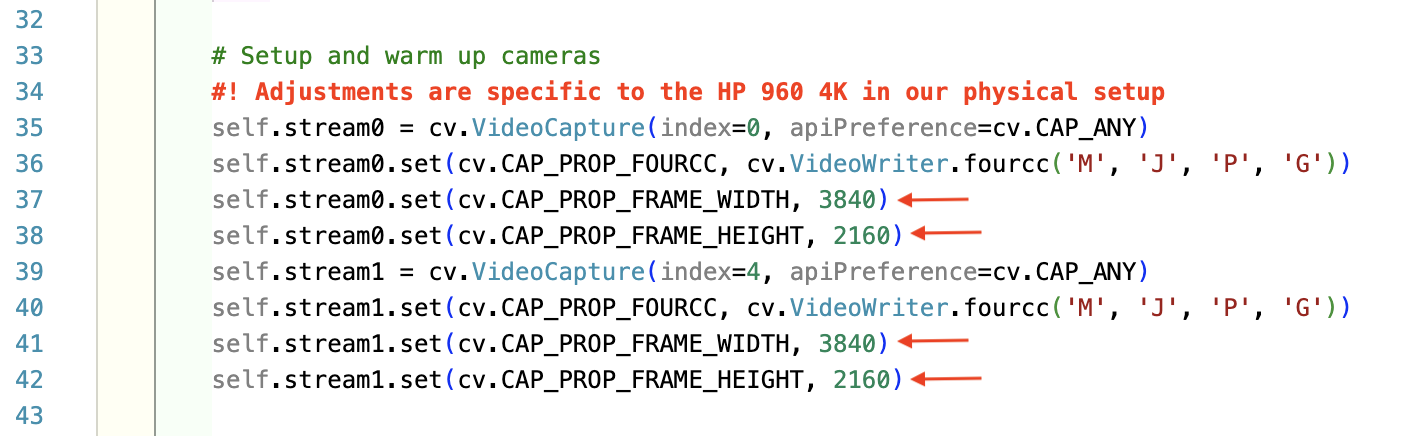
\includegraphics[width=\textwidth]{stream_properties.png}
\end{figure}


\section{Troubleshooting}
\label{sec:troubleshooting}

Um das Projekt über das Terminal zu starten, oder um Änderungen am conda environment vorzunehmen, muss das environment bei jedem Terminal neustart wieder aktiviert werden (\code{conda activate hybparc}).

\paragraph{OpenCV Package Type}
Das Guide empfiehlt \code{opencv-contrib-python} zu installieren. Dies ist eine Ubuntu Linux spezifische Empfehlung. Sollte das Projekt unter MacOS und Windows verwendet werden empfiehlt sich das Package \code{opencv-python}.

\end{document}